\documentclass{article}
\usepackage{graphicx}
\graphicspath{ {./grafiki/} }
\usepackage{transparent}
\usepackage[T1]{fontenc}
\usepackage[a4paper, total={15cm, 24cm}]{geometry}
\usepackage[polish]{babel}
\usepackage{amssymb}
\usepackage{amsmath}
\usepackage[
  pdfpagelabels=true,
  pdftitle={Notatki z OWI},
  pdfauthor={Jan Pulkowski},
  colorlinks=true,
  linkcolor=blue,
  ]{hyperref}
\usepackage[]{titlesec}
\usepackage[p]{scholax}

\newcommand{\watermark}{
  \begin{figure}[b]
    \transparent{0.4} \includegraphics*[]{mlecz}
    \centering
  \end{figure}
}

\setcounter{secnumdepth}{2}

\renewcommand{\thesection}{\arabic{section}}

\titleformat{\section}{\normalfont\Large\bfseries\scshape}{Wykład \thesection:}{1em}{}

\title{Notatki z Ochrony Własności Intelektualnej}
\author{mlecz}
\date{Semestr Letni 2024}

\begin{document}

\maketitle
\tableofcontents
\watermark

\newpage
\section{Prawo i jego źródła (28.02)}

\subsection{Prawo}

\paragraph{Prawo w ujęciu normatywnym}
to zespół norm i reguł określających postępowanie ludzi, ustanowionych, usankcjonowanych i zabezpieczanych przez aparat przymusu państwowego.

\paragraph{Prawo wg Kanta}
to reguły pozwalające na pogodzenie samowoli dwóch niezależnych jednostek.

\subsubsection{Zasady Prawa}
\begin{itemize}
  \item Lex posterior derogat legi priori -- prawo późniejsze uchyla prawo wcześniejsze
  \item Lex superiori derogat legi inferiori -- prawo o wyższej mocy uchyla prawo o niższej mocy
  \item Lex specialis derogat legi generali -- prawo szczegółowe uchyla prawo ogólne
  \item Ne bis in idem -- Nie można orzekać dwa razy w tej samej sprawie
  \item Lex retro non agit -- Prawo nie działa wstecz (o ile ustawa późniejsza nie jest
        korzystniejsza dla oskarżonego)
\end{itemize}

\subsubsection{Miejsca zapisu prawa}
\begin{itemize}
  \item \textbf{Dziennik ustaw -- jedyne oficjalne miejsce zapisu prawa}
  \item Monitor Polski -- służy do ogłaszania wewnętrznych aktów prawnych wydawanych
        przez organy państwowe
  \item ISAP -- Internetowy System Aktów Prawnych
  \item Systemy Prawne (LEX, Legalis) -- ujednolicony i czytelny zapis informacji
        z dziennika ustaw z odnośnikami do innych powiązanych informacji prawnych
\end{itemize}

\subsection{Język prawny a prawniczy}

\paragraph{Język prawny} to język tworzenia prawa, w którym tworzone są akty prawne.
Nie musi być poprawny w sensie składni j. pol. ale jest mniej wieloznaczny i ściślejszy
od języka naturalnego.

\paragraph{Język prawniczy} to język stosowania i doktryny prawa, omawiający treść
i interpretację ustawy.

\paragraph{Język prawny a matematyczny}
Język prawny często celowo zostawia pewne pojęcia niedookreślone,aby pozostawić
sądom pole do odmiennej wykładni prawa w różnych przypadkach.

\subsection{Obowiązywanie Prawa}

\paragraph{Prawo powszechnie obowiązujące} to przepisy adresowane do wszystkich podmiotów.
Wyznacza ich sytuację prawną, tzn. prawa i obowiązki.
Stanowi fundament działania państwa,
jest umową społeczną między jego państwa i obywatelami.
Państwo może wykonywać jedynie czynności \textit{explicite} dozwolone przez prawo,
a obywatele wszystkie czynności niezakazane.

\subsection{Źródła prawa}
\begin{enumerate}
  \item Konstytucja
  \item Ustawy
  \item Ratyfikowane umowy międzynarodowe
  \item Rozporządzenia
  \item Akty prawa miejscowego (tylko na obszarze obowiązywania)
\end{enumerate}

\paragraph{Konstytucja}-- akt prawny nadrzędny wobec wszystkich pozostałych.
Jej przepisy stosuje się bezpośrednio, o ile sama nie stanowi inaczej.
Jest jednym, spójnym aktem prawnym. Konstytucja jest celowo napisana w sposób ogólny, aby mogły
uszczegółowić ją ustawy.
Określa bazowe ramy prawne, sposób stanowienia prawa i zasady jakie można z niej wyprowadzać.

\paragraph{Ustawa, a rozporządzenie} -- Ustawa to prawo stanowione przez władzę ustawodawczą,
rozporządzenie jest aktem wykonawczym, doprecyzowuje działanie i stosowanie ustawy oraz określa
szczegółowe procedury jej realizacji. Rozporządzenia są tworzone na podstawie ustaw.

\subsection{Prawo unijne}

\paragraph{Prawo pierwotne}
to umowy międzynarodowe tworzące i kształtujące Unię Europejską. Stanowią jej swoistą konstytucję.
Na przykład Traktat z Lizbony powołujący Unię.

\paragraph{Prawo wtórne}
to rozporządzenia, dyrektywy, decyzje, opinie i zalecenia wydawane przez organy Unii.

\paragraph{Rozporządzenia unijne} to akty prawne
bezpośrednio i jednolicie działające we wszystkich krajach członkowskich.

\paragraph{Dyrektywy unijne} to akty prawne,
wskazujące cele i wytyczne, które ustawodawstwo poszczególnych krajów członkowskich powinno zrealizować.
Muszą zostać wydane krajowe akty prawne, które implementują dyrektywę.

\subsubsection{Prawo polskie a prawo unijne}
Konstytucja dopuszcza przekazanie części uprawnień organów państwowych organom prawa międzynarodowego.
Proeuropejska wykładnia prawa jest ponad krajową --
ratyfikowana umowa międzynarodowa ma pierwszeństwo wobec sprzecznej z nią ustawy.
Nad umowami międzynarodowymi stoi jedynie konstytucja.


\section{Własność Intelektualna (06.03)}

\subsection{Dobra Niematerialne}

\paragraph{Dobro niematerialne (intelektualne)}
to wytwór myśli, cechujący się twórczym charakterem, istniejący w świadomości człowieka
i mogący podlegać ochronie prawnej niezależnie od~swojego ewentualnego nośnika \textit{(Corpus Mechanicum)}.

\subsubsection{Rodzaje dóbr niematerialnych}
\begin{itemize}
  \item Utwory (w rozumieniu prawa autorskiego)
  \item Rozwiązania -- zaplanowane koncepty, prowadzące do realizacji danego celu (wynalazki, projekty, wzory)
  \item Oznaczenia, symbole (znaki towarowe, oznaczenia geograficzne)
\end{itemize}

Dobra niematerialne mogą obejmować więcej niż jeden z powyższych aspektów.

\subsection{Prawo własności intelektualnej}

\paragraph{Prawo autorskie i pokrewne}
zajmuje się utworami. Godzi prawa twórców z możliwością rozwoju społeczeństwa. Chroni prawa twórców jak i wykonawców. Regulowane międzynarodowo.

\subsection{Konwencje o ochronie prawa autorskiego}

\subsubsection{Konwencja Berneńska}

\paragraph{Konwencja Berneńska}
o ochronie dzieł literackich i artystycznych z 1886 roku. Powstała z~inicjatywy m. in. Wiktora Hugo.
Wprowadziła koncept międzynarodowej ochrony praw autora.
Ratyfikowana przez większość państw świata, wielokrotnie nowelizowana. Nadal obowiązuje.

\paragraph{Zasada wzajemnego respektowania praw} Utworom zagranicznym zapewnia się taką samą ochronę jak utworom krajowym.

\paragraph{Zasada automatyzmu}
Ochrona praw autorskich przysługuje każdemu utworowi od momentu jego powstania.

\subsubsection{Inne Konwencje}

\paragraph{Konwencja genewska} o prawach autorskich.
Zapewnia alternatywę wobec Konwencji Berneńskiej.
Reprezentuje bardzie liberalne podejście do sprawy.

\paragraph{Konwencja Rzymska}
o ochronie wykonawców, producentów fonogramów oraz organizacji nadawczych.
Zapewnia ochronę twórcom utworów dźwiękowych.

\paragraph{Porozumienie w sprawie Handlowych Aspektów Praw Własności Intelektualnej (TRIPS)}
poza zakresem Konwencji Berneńskiej zapewniło ochronę programów komputerowych i baz danych.
Chroni programy w postaci kodu źródłowego i przedmiotowego (postać binarna, wynikowa, ang. \textit{object files}).

\paragraph{Traktaty Światowej Organizacji Własności Intelektualnej (WIPO)}
o prawie autorskim, o artystycznych wykonaniach i fonogramach.
Pierwszy traktat międzynarodowy nakładający obowiązek chronienia programów komputerowych i baz danych.
Wymusza wprowadzenie sankcji za łamanie i obchodzenie zabezpieczeń programów.

\subsection{Ustawa o prawach autorskich i pokrewnych}

\subsubsection{Utwory}

\paragraph{Utwór} to każdy przejaw działalności twórczej o indywidualnym charakterze, ustalony w~jakiejkolwiek postaci,
niezależnie od wartości, przeznaczenia i sposobu wyrażenia.
Definicja celowo jest szeroka aby móc pozostawić kwestię, czy dana rzecz jest utworem do interpretacji sądowej.

\paragraph{Konkretne przypadki wykładni definicji utworu}
\begin{itemize}
  \item Smak i zapach nie może podlegać ochronie prawnoautorskiej. Subiektywne doznania odgrywają tu zbyt dużą rolę.
  \item By mówić o utworze konieczna jest cecha nowości, twórca musiał wprowadzić uchwytne elementy, nieobecne w dotychczasowym stanie rzeczy.
  \item Jeżeli wysoce prawdopodobne jest, że ktoś w przyszłości wytworzy \textbf{identyczny} przedmiot, to nie mówi się o utworze.
\end{itemize}

\paragraph{Zasada Ustalenia}
-- Utwór musi zostać przedstawiony, w postaci która pozwala na jego percepcję komuś innemu niż twórcy, nawet ulotnej, nietrwałej.
Utwór może istnieć bez nośnika, a posiadanie nośnika nie jest związane z prawem do utworu.

\section{Twórcy i ochrona utworów (13.03)}

\subsection{Osoba twórcy}

\paragraph{Twórcą}
utworu może być dowolna osoba, niezależnie od stanu świadomości.
W porządku prawnym amerykańskim i polskim przesądzono, że zwierzęta ani natura nie mogą być twórcą utworu.
Ogólnie, twórcą może być wyłącznie człowiek.
Często uważa się, że wytwory systemu niedeterministycznych (np. AI) należą do ich operatorów,
natomiast nie jest to uniwersalna wykładnia i silnie zależy od konkretnego przypadku.
Obecny porządek prawny niedostatecznie określa interpretacje praw do wytworów sztucznej inteligencji,
która nie może być uznana za~twórcę utworu.

\subsection{Ochrona utworów}

Utwór jest chroniony od momentu powstania, nawet w postaci nieukończonej.
Ochrona przysługuje mu niezależnie od spełnienia jakichkolwiek formalności.
Ochronie nie może podlegać procedura, koncepcja matematyczna ani odkrycia,
a jedynie sposób wyrażenia (nie temat a jego indywidualizacja).
Dyrektywy unijne i inne przepisy doprecyzowują kryteria uznania tworu konkretnego typu za utwór.

\paragraph{Czy każde dzieło jest chronione jako utwór?}
tldr.: Nie.
\begin{figure}[h]
  \begin{minipage}{0.32\textwidth}
    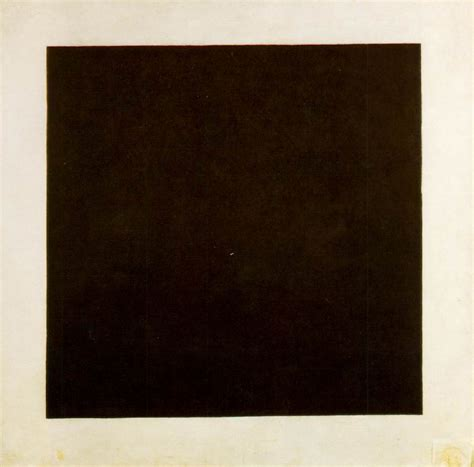
\includegraphics[width=0.95\textwidth]{malewiczkwadrat}
    \caption{K. Malewicz -- Czarny kwadrat na białym tle}\label{fig:malewiczkwadrat}
  \end{minipage}
  \begin{minipage}{0.32\textwidth}
    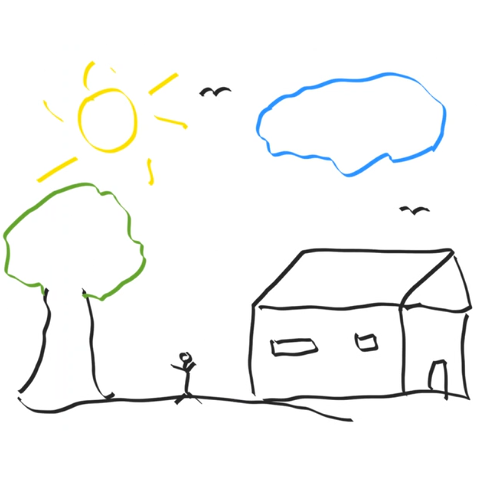
\includegraphics[width=0.95\textwidth]{behandomek}
    \vspace{-\baselineskip}
    \caption{A. Behan -- 2023}\label{fig:behandomek}
  \end{minipage}
  \begin{minipage}{0.32\textwidth}
    
\includegraphics[width=0.95\textwidth]{iosononiewidzialne}
    \vspace{-\baselineskip}
     \caption{S. Garau -- Io Sono}\label{fig:iosononiewidzialne}
  \end{minipage}
\end{figure}

Z powyższych utworem jest tylko Rysunek 2.
Niewidzialna rzeźba (3) istnieje jedynie jako koncepcja, nie ma żadnej ustalonej formy -- nie jest utworem.
Natomiast czarny kwadrat (1) pomimo oryginalnej koncepcji, nie spełnia kryterium oryginalności.
Prawdopodobieństwo wytworzenia identycznego dzieła jest zbyt duże by mówić o utworze.

\subsection{Ochrona programów komputerowych}

\paragraph{Programy Komputerowe}
podlegają ochronie w każdej postaci (kod, kod skompilowany, zapis na nośniku).
Programy chronią też wystarczająco szczegółowe prace przygotowawcze i projektowe.
Ochrona to nie zależy od testów jakościowych ani estetycznych programu, ani od jego oryginalności.
Programy komputerowe są chronione w taki sam sposób co dzieła literackie.
Nie są chronione ich koncepcje i interfejsy (graficzne/tekstowe).
Pojedyncze elementy programów mogą być chronione z osobna.
Np. interfejs graficzny może być objęty ochroną utworu, ale osobno od ochrony samego programu komputerowego.

\subsubsection{Dekompilacja Programów Komputerowych (10.04)}

\paragraph{Interfejs}

logiczna lub fizyczna część systemu informatycznego, służąca komunikacji z jego innymi częściami i użytkownikami.

\paragraph{Interoperacyjność}

umożliwienie połączenia, współpracy i oddziaływania pomiędzy interfejsami.
Zdolność do wymiany informacji i wykorzystania informacji już wymienionych.

\paragraph{Dekompilacja}

tłumaczenie formy programu komputerowego do wersji wyższego poziomu, termin nie jest jednoznaczny z informatycznym. Jest dozwolona jeżeli służy osiągnięciu interoperacyjności danego programu z innymi.

\paragraph{Kto może dekompilować?}

Osoba będące licencjobiorcą, posiadające prawo do używania kopii programu, lub działająca w imieniu takich osób.

\paragraph{Kiedy można dekompilować?}

Gdy informacje konieczne do osiągnięcia interoperacyjności nie są łatwo dostępne i nie jest na celu naruszenie uzasadnionych interesów twórców programu ani wykorzystanie programu w celach innych niż standardowe.
Poprawienie błędu i~naprawy są uzasadnionym powodem.
Nie jest wymagane zezwolenie autora i nie wolno zabraniać napraw.


\section{Autorskie prawa zależne (20.03)}

\subsection{Utwory zależne}

Opracowania utworów pierwotnych takie jak tłumaczenia, przeróbki, adaptacje.
Można je tworzyć i rozpowszechniać za zgodą pierwotnego twórcy.
Wytworzenie ich jest bez uszczerbku dla~praw pierwotnych i pociąga za sobą prawa autora utworu zależnego.
Należy zaznaczyć, że~jest to utwór pierwotny i wymienić twórcę i tytuł utworu pierwotnego.
Aby wytworzyć utwór zależny należy uzyskać zgodę autora pierwotnego, o ile jego prawa nie wygasły.

\paragraph{Tłumaczenia}

nie zawsze noszą cechy utworów - tłumaczenia które mają w sobie mało inwencji,
jak np. tłumaczenia dokumentacji technicznej nie są utworami, w przeciwieństwie do~tłumaczeń dzieł literackich.

\paragraph{Utwory zależne a inspirowane}

Utwór inspirowany to taki, który zawiera pewne motywy zawarte w innym utworze.
Jeżeli motywy są zindywidualizowane do postaci zawartej w utworze pierwotnym, to nie jest to już utwór inspirowany.
Utwory inspirowane nie są utworami zależnymi

\section{Utwory niechronione prawem autorskim (10.04)}

Poniższe kategorie utworów są niechronione prawem autorskim.
Mogą natomiast być chronione jako symbole narodowe, znaki towarowe bądź przez inne akty prawne.

\begin{itemize}
  \item akty normatywne i ich projekty.
  \item urzędowe dokumenty, materiały, znaki i symbole
  \item opublikowane opisy patentowe, lub ochronne
  \item proste informacje prasowe
\end{itemize}

Nie wszystkie materiały tworzone przez urzędy to materiały urzędowe.
Na przykład dokumenty wytworzone na potrzeby przetargów, jak najbardziej są chronione prawem autorskim.

\end{document}
